\documentclass[review]{elsarticle}

\usepackage{lineno,hyperref}
\usepackage{algorithm}
\usepackage{algorithmic}
\usepackage{subfigure}
\usepackage{mathtools}
\usepackage{graphicx}
%\usepackage{rotating}

\modulolinenumbers[5]

\journal{Journal of \LaTeX\ Templates}


\bibliographystyle{elsarticle-num}


\begin{document}

\begin{frontmatter}

\title{A Novel Clustering Method using Enhanced Grey Wolf Optimizer and MapReduce}

\author{Ashish Kumar Tripathi}

\author{Kapil Sharma*}
\cortext[mycorrespondingauthor]{Corresponding author}
\ead{kapil@ieee.org}
\author{Manju Bala}
\begin{abstract}
 With advancement of the technology, data size is increasing rapidly. For making intelligent decisions based on data, efficacious analytic methods are required. Data clustering, a prominent analytic method of data mining, is being efficiently employed in data analytics. To analyze massive data sets, the improvement in the traditional methods is the urge of todays scenario. 
 In this paper, an efficient clustering method, MapReduce based enhanced grey wolf optimizer (MR-EGWO), is presented for clustering large-scale data sets. The proposed method introduced a novel variant of grey wolf optimizer, Enhanced grey wolf optimizer (EGWO), where the hunting strategy of grey wolf is hybridized with binomial crossover and l\'{e}vy flight steps are inducted to enhance the searching capability for pray. Further, the proposed variant is used for optimizing the clustering process. The clustering efficiency of the EGWO is tested on seven UCI benchmark datasets and compared with the five existing clustering techniques namely K-Means, particle swarm optimization (PSO), gravitational search algorithm (GSA), bat  algorithm (BA) and grey wolf optimizer (GWO). The convergence behavior and consistency of the EGWO has been validated through the convergence graph and boxplots. Further, the proposed EGWO is parallelized on the MapReduce model in the Hadoop framework and named MR-EGWO to handle the large-scale datasets. Moreover, the clustering quality of the MR-EGWO is also validated in terms of F-measure and compared with four MapReduce based state of art namely: parallel K-Means, parallel K-PSO, MapReduce based artificial bee colony optimization (MR-ABC), dynamic frequency based parallel k-bat algorithm (DFBPKBA). Experimental results affirm that the proposed technique is promising and powerful alternative for the efficient and large-scale data clustering.
\end{abstract}

\begin{keyword}
Clustering method  \sep grey-wolf optimizer \sep Hadoop \sep and MapReduce 
\end{keyword}

\end{frontmatter}



\section{Introduction} \label{sec:intro}

 Clustering is the prominent approach of unsupervised learning and considered as part and parcel of data engineering applications, such as  image segmentation, data mining, information retrieval system, anomaly detection, medicine, computer vision and construction management \cite{fayyad2002information, friedman2007anomaly, liao2008mri, forgy1965cluster}. Over the past years, several algorithms for data clustering have been introduced in the literature to handle the diversity in data and different sets of application requirements. K-means, one of the simplest and popular algorithm, has been employed for unfolding the various clustering problems \cite{xu2005} \cite{kaufman2009finding}. However, the results of K-means algorithm are highly dependent on initial cluster centroids and it probability of trapping into local optima is high \cite{kao2008hybridized}.

   To mitigate this issue, various metaheuristic-based clustering methods have been proposed in literature. Maulik et al. \cite{maulik2000genetic} used the ability of genetic algorithm to find the best centroid in the feature space so that the compactness of the resulting clusters is optimized. Sharma et al. \cite{ashish2018parallel} proposed bat algorithm based method for optimizing the clustering process. The proposed method was also parallelized using MapReduce to handle large data sets. Hatamlou et al. \cite{hatamlou2012combined} introduced gravitational search algorithm based clustering method which used K-means algorithm for initializing the center heads. Karaboga et al. \cite{karaboga2011novel} proposed a novel artificial bee colony based method for clustering the multivariate data. Kumar et al. \cite{kumar2017grey} introduced a clustering algorithm which imitate the hunting behavior of grey wolves. Cura et al. \cite{alam2008particle} developed particle swarm optimization based clustering method and solved the web application problems. However, the above clustering algorithms fail to perform efficiently on large datasets in terms of memory space and the time complexities due to their sequential execution. 

For alleviating computation performance on large dataset, parallel and distributed computation has exhibited attractive solutions. With the years of progress in parallelization tools, apache hadoop is a widely used parallelization tool. Hadoop \cite{shvachko2010hadoop} is an open source platform, as developed managed by Apache for handling large datasets using distributed processing. Hadoop works with its own file system referred as HDFS (hadoop distributed file system) and, is capable of processing zeta bytes of data with commodity hardware \cite{FrontPag86:online} .
MapReduce \cite{dean2008mapreduce}provides the parallel computation platform and has successfully leveraged the strengths of meta-heuristics algorithms for analyses of large-scale datasets \cite{khezr2015mapreduce, wang2012parallel, lin2013parallelizing}. Gong et al. \cite{gong2015distributed} studied the different distributed evolutionary models and appreciated the simplicity of MapReduce architecture for solving various computation intensive problems. Thus, researchers have worked upon MapReduce based parallel meta-heuristic algorithms in the last five years. 
      A hybrid K-PSO method with MapReduce architecture was proposed by Wang et al. \cite{wang2012parallel} to cluster massive datasets.
 Banharnsakun \cite{banharnsakun2016mapreduce} proposed MapReduce based artificial bee colony algorithm (MR-ABC) for clustering large datasets.
Tripathi et al. \cite{tripathidynamic} proposed dynamic frequency base K-Bat algorithm for handling massive datasets (DFBPKBA). In the proposed method, the frequency of the bats was dynamically changed to improve the clustering accuracy and MapReduce architecture was used to handle large datasets. 
  Zhao et al. \cite{zhao2009parallel} were successful in mining knowledge from the big data through the parallel version of K-Means algorithm.
   Khezr et al. \cite{khezr2015mapreduce} studied various distributed models of the nature inspired algorithms and concluded that the Hadoop MapReduce model is one of the widely used platform for the parallel processing of large datasets due to simplicity and robustness. As ‘‘No free lunch’’ theorem \cite{wolpert1997no} obviates the claim of Idle meta-heuristic algorithm for all set of optimization problems, this paper utilizes the merits of GWO to cluster massive datasets in parallel.

The grey wolf optimizer (GWO), proposed by Mirjalili et al. \cite{mirjalili2014grey}, is a swarm based meta-heuristic algorithm and is inspired by the hunting behavior of Grey wolfs. It has outperformed well-designed meta-heuristics such namely particle swarm optimization (PSO), evolution strategy (ES), gravitational search algorithm (GSA), differential evolution (DE) for on standard benchmark problems[23]. Further, Emary et al. \cite{emary2016binary} proposed the binary version of GWO and performed the optimization of feature selection. Komaki and Kayvanfar \cite{komaki2015grey} optimized the flow shop scheduling tasks by applying GWO. Song et al. \cite{el2015single} unfolded GWO for the optimal tuning of the surface waves parameters. Moreover, GWO has also been applied for solving the power dispatch and mixed heat task for power systems \cite{jayakumar2016grey}. Medjahed et al. \cite{medjahed2016gray} introduced a GWO-based method for selection of hyperspectral bands. Fergany and Hasanien \cite{ho2002simple}, demonstrated the efficiency of GWO on optimal power flow (OPF) problem. On the same footnote, GWO was drafted to design the wide area power system stabilizer (WAPSS) \cite{shakarami2016wide}. To solve the economic dispatch problem, Jayabarathi et al. \cite{jayabarathi2016economic} introduced mutation and crossover mechanisms in GWO. D. Guha \cite{guha2016load} employed GWO in power systems for optimizing the load frequency control (LFC). 
   Despite of wide applicability, GWO has limitation of lack of population diversity. This results in slow convergence rate and risk of trapping into local optima \cite{zhang2015grey}. To improves its search precision, a novel variant of GWO, Enhanced grey wolf optimizer (EGWO), is proposed in this paper by incorporating the following capabilities. 
\begin{itemize}
\item  L\'{e}vy Flight steps: To magnify search for prey.
\item Binomial crossover: To inflate the attack to pray. 
\end{itemize}
  The overall contribution of this paper has been divided into three folds. First, a novel clustering method is proposed based on the new variant of GWO. Second, the efficiency of proposed variant is studied on clustering problem. Third, the proposed method is parallelized using MapReduce architecture and named MR-EGWO for efficacious clustering of large datasets. The empirical analysis of EGWO has been done on seven UCI datasets and validated against five clustering algorithms namely K-Means \cite{xu2005}, PSO \cite{alam2008particle}, GSA \cite{hatamlou2012combined}, BA \cite{ashish2018parallel} and GWO \cite{kumar2017grey} in terms of Mean and Best of intra cluster distance. The convergence behavior of EGWO is discussed along with the box plots to visualize its consistency. Moreover, the clustering performance of MR-EGWO is also validated in terms of F-measure by comparing with four MapReduce based parallel state of art namely:PK-Means, parallel K-PSO, MR-ABC, DFBPKBA. To demonstrate the parallel computation performance, the proposed method (MR-EGWO) has been analyzed on four large scale datasets and asserted through speedup graphs.

The remainder of this paper is organized as follows. Section \ref{sec:bg} briefs the basics of clustering and GWO algorithm. In section \ref{sec:pm}, the clustering process using the proposed algorithm along with its parallelization using MapReduce is explained. Section \ref{sec:ep} explains the experimental environment settings and the simulation results. Finally, the paper in concluded in section \ref{sec:con}.
\section{Background}\label{sec:bg}

     \subsection{Data Clustering Approach}
  Clustering of a dataset in t-dimensional space is the process of assembling of $N$ data objects into $K$ groups on the basis of resemblance \cite{banharnsakun2016mapreduce}. Clustering partitions the data objects iteratively into $K$ groups(clusters) in such a way, that the data objects within the same group have maximum resemblance. Further, data clustering is a type of unsupervised learning approach, that means data objects are grouped on the basis of structure of the data, without any training. Whereas, in supervised learning like classifications, data objects are classified based on the training set using labeled data.
    The proposed EGWO performs clustering with the known number of clusters. The summation of intra-cluster distance of $K$ clusters is chosen as the criterion for the evaluation of the quality of the clustering. 
Let $Z={(z_1, z_2, z_3, \cdots, z_n)}$ is a collection of $N$ data objects where all the data object are represented in $t$ dimensional space. The data objects are represented by a matrix of $Z_{n\times t}$ having $n$ rows and $t$ columns where each row vector describes one data object. The clustering process allocates the set of $N$ data objects to $K$ clusters and find a set of cluster centroids, $C={\{C_1,C_2, \cdots ,C_k\}}$ with the aim of minimizing the sum of squired euclidean distance between each data object $Z_i$ and its centroids $C_i$ to which it belongs. Generally, clustering process satisfies the following properties: 
\begin{itemize}
\item Each and every cluster must have at minimum one data object, i.e., $C_i \neq \phi , \forall i\in \{1,2,3, \cdots,k\}$.
\item Each data object certainly be part of a cluster.
\item No data object can be part of more than one cluster, i.e., $C_q \cap C_r=\phi,\forall q\neq r$ and $q,r \in \{1,2,3,\cdots,k\}$.
\end{itemize}   
A dataset is grouped based on the above three conditions and the quality of clustering is evaluated in terms of the fitness value. The sum of squared Euclidean distance \cite{yang2010evolutionary}is one of the famous function used for the evaluating the quality of the clustering, which is calculated using Eq. (\ref{eq:25}).
   \begin{equation}\label{eq:25} 
   f(Z,C)=\sum_{l=1}^k\sum_{Z_i\epsilon C_l}d(Z_i,C_l)^2
   \end{equation}
where $d(Z_i,C_l)$ is the measure of diversity between the data object $Z_i$ and centroid of the cluster $C_l$. For calculating the dissimilarity between data objects, many distance metrics have been proposed. Euclidean distance is one of the popular distance metric available to compute the dissimilarity between the data objects. Given two data objects $Z_i$ and $Z_j$ with $t$ dimensions, the euclidean distance $d(Z_i,Z_j)$ is calculated as by equation Eq. (\ref{eq:26}).
   \begin{equation}\label{eq:26}
     d(Z_i,Z_j)=\sqrt{\sum_{t=1}^t(z_i^t-z_j^t)^2}
   \end{equation}
  \subsection{Grey wolf optimizer }\label{sec:GWO}
 Grey wolf optimizer (GWO) is a meta-heuristic algorithm proposed by Mirjalili et al. \cite{mirjalili2014grey} which imitate the hunting mechanism of the grey wolves. 
In GWO, grey wolves are grouped into $alpha(\alpha)$, $beta(\beta)$, $delta(\delta)$ and $omega(\omega)$ according to their social hierarchy. The best three grey wolves are considered as $alpha$, $beta$, $delta$ and renaming grey wolves are termed as $omega$. The $alpha$ wolves are the commanding one and all other grey wolves follows their instructions. The second category of the wolves belonging to the $Beta$ category are responsible for helping $alpha$ in their decision making. $Omega$ are the lowest ranked grey wolves.\newline
     In the grey wolf algorithm, hunting is escorted by $alpha$, $beta$ and $delta$ while $omega$ wolves are responsible for encircling the prey to find better solution.
   The encircling operation performed by the grey wolves is mathematically defined by Eq. (\ref{eq:3}) and (\ref{eq:4}):


 \begin{equation}\label{eq:3}
    \overrightarrow D=|\overrightarrow C.\overrightarrow X_p(i)-\overrightarrow X(i)|                           
\end{equation}   
 \begin{equation}\label{eq:4}                               
   \overrightarrow X(i+1)=\overrightarrow X_p(i)+\overrightarrow A.\overrightarrow D
\end{equation}

     where $X_p$ is the location of the prey, $X(i)$ is the location of the grey wolf at $i^{th}$ iteration. $\overrightarrow A$, and $\overrightarrow C$ are coefficient vectors and computed using Eq. (\ref{eq:5}) and (\ref{eq:6}) respectively. 
 \begin{equation}\label{eq:5}                                             	
       \overrightarrow A=2 \overrightarrow a. \overrightarrow {r_1}-a.                                                     	
   \end{equation}
   \begin{equation}\label{eq:6} 
   \overrightarrow C=2. \overrightarrow {r_2}.
    \end{equation} 
  	 where $\overrightarrow a$ is coefficient vector which is reduced linearly from 2 to 0 with the increasing number of iterations and $r_1$, $r_2$ are the random numbers between [0,1]. 

     \begin{equation}\label{eq:7}
    \overrightarrow D_{\alpha}=|\overrightarrow C_1.\overrightarrow X_{\alpha}-\overrightarrow X|                           
\end{equation} 
 \begin{equation}\label{eq:8}
    \overrightarrow D_{\beta}=|\overrightarrow C_2.\overrightarrow X_{\beta}-\overrightarrow X|                          
\end{equation} 
 \begin{equation}\label{eq:9}
       \overrightarrow D_{\delta}=|\overrightarrow C_3.\overrightarrow X_{\delta}-\overrightarrow X|                          
\end{equation} 

 Further, Eqs. (\ref{eq:7}), (\ref{eq:8}) and (\ref{eq:9}) define the estimated span around the current position and $alpha$, $beta$ and $delta$, respectively.
After estimating of distances, the final position of the $\omega$ wolves is determined by Eq. (\ref{eq:10}). Where, $\overrightarrow A_1$, $\overrightarrow A_2$, $\overrightarrow A_3$ represents the random vectors and $i$ shows the current iteration number. 
\begin{equation}\label{eq:10}
        \overrightarrow X(i+1)=\left[ \frac{\overrightarrow X_1+\overrightarrow X_2+\overrightarrow X_3} {3}\right]     
\end{equation} 
where, $\overrightarrow X_1$, $\overrightarrow X_2$, $\overrightarrow X3$, are defined by Eq. (\ref{eq:11}), (\ref{eq:12}), and (\ref{eq:13}) respectively.
 \begin{equation}\label{eq:11}
    \overrightarrow X_1=\overrightarrow X_{\alpha}-A_1.D_{\alpha}      \end{equation}                     
 \begin{equation}\label{eq:12}
    \overrightarrow X_2=\overrightarrow X_{\beta}-\overrightarrow A_2.\overrightarrow D_{\beta}      \end{equation}                     
 \begin{equation}\label{eq:13}
       \overrightarrow X_3=\overrightarrow X_{\delta}-\overrightarrow A_3.\overrightarrow D_{\delta}        \end{equation}              


      \section{Proposed Method}\label{sec:pm}
     To deal the problems of large dataset clustering, a novel method, Map-reduce based enhanced grey wolf optimizer (MR-EGWO), is proposed. MR-EGWO leverages the strengths of a novel variant of grey wolf optimizer, enhanced grey wolf optimizer (EGWO), for efficient data clustering. In this section, first a detailed description of the enchanced grey wolf optimizer (EGWO) is presented followed by its parallel version, Map-reduce echanced grey wolf optimizer (MR-EGWO) is discussed.

     \subsection{Enhanced Grey Wolf Optimizer (EGWO) }  \label{sec:EGWO} 
    
    The success of a meta-heuristic algorithm depends upon the equilibrium between exploration and exploitation \cite{feoktistov2007differential}. The GWO algorithm has limitations of slow convergence rate and risk of trapping into local optima due to the lack of diversity in the wolves for certain cases \cite{zhang2015grey}. These limitations can be overcome by the increase of diversification and intensification of the search space.
Therefore, in this paper a novel variant of GWO named enhanced grey wolf optimizer (EGWO) is proposed. The proposed method is empowered with the advantages of l\'{e}vy \cite{yang2010eagle} flights and binomial crossover \cite{feoktistov2007differential} to improve the exploration and exploitation capabilities. 
   The EGWO introduces two new phases to relieve the above mentioned problem.
      \subsubsection{Inflated Attack to pray using Binomial Crossover} \label{sec:binomial}
      
    As the intensification of the population around the current best solution inflates the generation of optimal solutions. The exploitation in the proposed variant is enhanced by including one of the popular and widely used binomial crossover operator present in the literature. As $alpha$ wolf defines the current best position, its position can be used to define the better position of other wolfs. Hence, binomial crossover operator is performed between between the $alpha$ and the $X(i)$ to inflate the attack to the pray. The updated position (UP) of grey wolves is defined in Eq. (\ref{eq:18}). 
                                 \begin{equation}\label{eq:18}
                     UP_i^j=\begin{cases}\overrightarrow X_{\alpha}^j &  (K\leq C)\\{\overrightarrow X_i^j} &  (K>C)\end{cases}
               \end{equation}
   Where $UP_i^j$ is the position of the $i_{th}$ grey wolf in $j^{th}$ dimension, $K$ is the random number between [0,1]. $C \in [0,1]$ is crossover constant.      
               \subsubsection{Magnified search for pray using on l\'{e}vy flight} \label{sec:levy}
  
In GWO, the problem of stagnation still prevails in some cases sine the position updation of a wolf is determined solely by the positions of leader wolves namely, alpha, beta, and delta. Correspondingly, GWO results in immature convergence. To enhance the exploration capability, the proposed EGWO uses the concept of l\'{e}vy flight to update the position of each wolf. As l\'{e}vy flight defines steps of random lengths drawn from the l\'{e}vy distribution \cite{shlesinger1995levy}, the chance of exploring the search space increases. This paper uses the Mantegna algorithm \cite{yang2010eagle} to generate steps of random length. The Eq. (\ref{eq:35}) depicts the formulation of step length $z$ defined by Mantega's algorithm.
             
         \begin{equation}\label{eq:35}
               z= \left[  \frac{r}{\mid s \mid ^{1/ \beta}} \right]
\end{equation}    
             where, $\beta \in (0,2]$ is l\'{e}vy index and $r$ and $s$ are variables following normal distribution of  $N(0, \sigma_{r}^2)$ and $N(0, \sigma_{s}^2)$, respectively. The  $\sigma_r$ is calculated by Eq. (\ref{eq:17}) while  $\sigma_s$ is  always $1$. 
 \begin{equation}\label{eq:17}
               \sigma_r=	\left[ \frac{ \Gamma(1+\beta)\sin(\pi\beta/2)  }   { \beta\Gamma[(1+\beta)/2]2^{(\beta-1)/2} } \right] ^{1/\beta}
        \end{equation} 

where, $\Gamma$(.) is called Gamma function and defined by Eq. (\ref{eq:16}).

        \begin{equation}\label{eq:16}
                  \Gamma(1+\beta)= \int_{0}^{\infty} t^\beta e^{-t} dt                     
        \end{equation} 

        In the proposed phase, each grey wolf takes l\'{e}vy flight for the search of the prey and updates its position using Eq. (\ref{eq:28}).   
     
                                                  \begin{equation}\label{eq:28}
                                                   \overrightarrow X_{t+1}=\overrightarrow X_t+estep_t
                                                \end{equation}

where, $\overrightarrow X_t$ is the position of the grey wolf at $t^{th}$ iteration, $\overrightarrow X_{\alpha}$ represents the position of $alpha$ wolf and $estep_t$ at a particular iteration $t$ defines the l\'{e}vy flight step size and calculated by Eq. (\ref{eq:27}).
\begin{equation}\label{eq:27}
                                                   estep_t=0.01\times(\overrightarrow X_t-\overrightarrow X_{\alpha});
                                                \end{equation}
\subsection{EGWO based clustering}
Furthermore, the proposed enhanced grey wolf optimizer (EGWO) is elucidated for  the clustering problem. In EGWO based clustering, the position $X$ of each grey wolf represents a set of cluster centroids ${(C_1,C_2,C_3, \cdots, C_K)}$ for $K$ clusters.  The minimization of intra-cluster distance is considered as the cost function and formulated in Eq. (\ref{eq:ob}).
\begin{equation}\label{eq:ob}
      f(Z,C)=\sum_{l=1}^k\sum_{Z_i\epsilon C_l}d(Z_i,C_l)^2
\end{equation}
The optimal clusters corresponds to the position of the $Alpha$ wolf. The pseudo-code of the EGWO based clustering method is described in Algorithm \ref{algo:EGWO}. 

 \begin{algorithm}
%\scriptsize
\caption{:Enhanced Grey Wolf Optimizer based clustering}
\label{algo:EGWO}
\begin{algorithmic}
\STATE\textbf{Input:} Data file having $Z$ data objects with $t$ dimensions and $K$ Number of clusters .
\STATE\textbf{Ouput:} Final centroids position.           /* The location of $\alpha$ after termination of algorithm represents centroids position*/
\STATE Generate initial population of $N$ grey wolves.
\STATE Initialize parameters $a$, $i$, $A$, $C$, maximum number of iteration $MaxItr$.
\STATE  Evaluate the fitness of each grey wolf using Eq. (\ref{eq:25}).
\STATE Set top three grey wolves according to the fitness as $\overrightarrow X_{\alpha}$, $\overrightarrow X_{\beta}$ and $\overrightarrow X_{\delta}$.
\WHILE{$(MaxItr) \ or \ (centroid \ movement \ becomes \ zero)$}
  \FOR {each grey wolf}
  \STATE Update the position of each grey wolf defined by Eq. (\ref{eq:10})
   \STATE Perform binomial cross over determined by Eq. (\ref{eq:18}).
  \STATE Determine the new position of each grey wolf using l\'{e}vy flight defined by Eq. (\ref{eq:28}).
  \STATE Upgrade the values of $a$, $A$, $C$.
  \STATE Calculate the fitness of each grey wolf.
  \STATE Update $\overrightarrow X_{\alpha}$, $\overrightarrow X_{\beta}$, and $\overrightarrow X_{\delta}$.
    \ENDFOR
\STATE  $i=i+1$; 
\ENDWHILE
\STATE Return $\overrightarrow X{\alpha}$  //the position of alpha is the final centroid position
\end{algorithmic}
\end{algorithm}

  \subsection{Parallelization of the EGWO using MapReduce Architecture}\label{sec:mpr}
To demonstrate the applicability of EGWO on large dataset, a parallel version of EGWO algorithm using Hadoop MapReduce framework, MapReduce based EGWO (MR-EGWO), is presented. MR-EGWO works in two phases; EGWO-Map and EGWO-Reduce. 
Initially, MapReduce framework divides the large datasets into smaller chunks of key/value pairs and distribute them uniformly among the hadoop nodes. The MR-EGWO map phase, then, processes the input key/value pairs with cluster centroids in  parallel and the corresponding fitness computation. The pseudo-code of the MR-EGWO Map phase is presented in Algorithm \ref{algo:Map}. The output of this phase is the another set of key/value pair where key consists of  $\{gwoID,centroidID\}$ while the intra-cluster distance with the respective centroid-ID defines the value component. Further, the reduce function of the MR-EGWO reduce phase merges all the computed values with identical key's and computes the corresponding fitness value for each grey-wolf. Algorithm \ref{algo:Reduce} presents the pseudo-code of the EGWO-reduce function. The $alpha$, $beta$, and $delta$ wolves are updated along with the position of each grey wolf according to the EGWO  \ref{algo:EGWO}.
This marks one iteration of the MR-GWO and is continued until the stopping criterion is reached. The complete architecture of the MR-EGWO for data clustering is shown in Fig. \ref{fig:EGWO}.   

      \begin{figure}
    \centering
     \includegraphics[width=1.0\textwidth]{algo}
      \caption{MapReduce architecture MR-EGWO for data clustering}
\label{fig:EGWO}
\end{figure}

\begin{algorithm}
\caption{ :MR-EGWO Map}
\small
\label{algo:Map}
\begin{algorithmic}
\STATE Map (Key: recordId, Value: Record)
\STATE \textbf{Initialization:}
\STATE  key=record-ID
\STATE  value=record
\STATE  read(gwoPopulation);
\STATE    \textbf{for each} wolf \textbf{in} gwo-population;
\STATE       gwoID   =retrieve-gwoID(gwoPopulation)
\STATE       centroidArray =retrieve-centroids(gwoPopulation)  / wolf position represents centroids 
\STATE   	minDistance= getMinD(record, centroidArray);     / getMinD returns minimum distance  
\STATE       centroid-ID =   i    / i represents index of the centroidArray having minimum distance
\STATE         updated-key= gwoID+centroidID;
\STATE      \textbf{end for}
  \STATE         write (updated-key, minDistance);
\end{algorithmic}
\end{algorithm}

\begin{algorithm}
\caption{ :MR-EGWO Reduce}
\small
\label{algo:Reduce}
\begin{algorithmic}  
\STATE \textbf{Reduce (Key:(gwoID, centroidID), value-list: minDistance)} 
\STATE  \textbf{Initialization} 
\STATE   fitness=0;
\STATE	\textbf{for each} value \textbf{in} minDistance list
\STATE	 minDistance=retrieve-minDistance(value-list)       
\STATE   fitness=+minDistance
\STATE   \textbf{end for}
\STATE    write(key, fitness)
\end{algorithmic}
\end{algorithm}

\section{Experimental results }\label{sec:ep}
The proposed work is evaluated in two folds. First, EGWO is validated for clustering in terms of intra-cluster distance and convergence behavior. The comparison is made with k-means and four meta-heuristic algorithms for clustering namely; GSA, PSO, BA, and GWO. Second, the effectiveness of the MapReduce based MR-EGWO is vindicated in terms of F-measure against the four state-of-the-art MapReduce based clustering methods namely parallel K-means (PKmeans) \cite{zhao2009parallel}, parallel K-PSO based on MapReduce (parallel K-PSO) \cite{wang2012parallel}, MapReduce based artificial bee colony optimization for large scale data clustering (MR-ABC) \cite{banharnsakun2016mapreduce} and Dynamic frequency based parallel K-Bat algorithm (DFBPKBA) \cite{tripathidynamic}. The speedup behavior of MR-EGWO is also studied by incrementing number of nodes in each run.  

\subsection{Performance analysis of EGWO based clustering}\label{sec:expr1}
The proposed EGWO algorithm is tested on seven benchmark datasets taken from UCI repository \cite{blake1998uci} and results are compared with K-means, PSO, GSA, BA and GWO. Table \ref{tab:dataset} detailed the seven considered benchmark datasets. The simulation is carried out for 30 runs on a system with Matlab 2015a, intel core i3 processor, $2.80 GH_z$ frequency, 4 GB of RAM and 500 GB hard-disk. Table \ref{tab:Param} details the parameter setting of the experimentation.  

\begin{table}
\caption{Parameter values}
\scriptsize
\begin{center}
\renewcommand{\arraystretch}{.75}
  \begin{tabular}{l l l l}
   
    \hline
\textbf{Dataset} & \textbf{NOC} & \textbf{NOF} &\textbf{NOI}    \\

\hline
Iris	      &	3	&	 4   &	150	\\
Wine	&	3	&	13	&	178	\\
Seeds	&	3	&	7	&	210	\\
Glass	&	6	&	9	&	214	\\
Cancer	&	2	&	9	&	638	\\
Balance	&	3	&	4	&	625	\\
Haberman	&	2	&	3	&	306	\\


    \hline
\multicolumn{4}{l}{NOC:Number of Clusters}\\
\multicolumn{4}{l}{NOF:Number of Features}\\
\multicolumn{4}{l}{NOI:Number of Instances}\\
  \end{tabular}
\end{center}
\label{tab:dataset}
\end{table}


  Table \ref{tab:result} defines the best and average fitness values attained by considered algorithms over 30 runs. It can be observed from the Table \ref{tab:result} that EGWO outperformed all five methods on all the datasets in terms of best fitness value. For average fitness value, EGWO has surpassed results for wine, seeds, glass and cancer. However, GWO has competitive results on Iris and Balance datasets while PSO performed well on Haberman dataset.
\begin{table}
\caption{Parameter values}
\scriptsize
\begin{center}
\renewcommand{\arraystretch}{0.7}
  \begin{tabular}{l l l l l l l}
    \hline
    \hline
\textbf{Parameter Name} & \textbf{K-Means} &\textbf{PSO} &\textbf{GSA} &\textbf{BAT}& \textbf{GWO} &\textbf{EGWO}\\
\hline
Population size (pop)	&	--& 40	&	40 &	40	&	40	&40\\
Number of Iterations (itr) &	500	&	500 &	500	&	500 & 500 & 500\\
Inertial Constant (w)	&	--& 0.5& --&	--	&	--&--	\\
Congnitive Constant (c1)	&	--& 1 & --&	--	&	--&--	\\
Social Constant (c2)	&--& 1 & --&	--	&	--&--\\
Gconstant (G0)&--& --& 20 & --&	--&--\\
Alpha ($\alpha$) --& 20& --&	.9 & 2&2 &--\\
fmin	&	--& --& --& 0	&	--&--\\
fmax	&	--& --& --&	2	&	--&--	\\
gamma ($\gamma$)& --& --& --&	.9	&	--&--	\\
r0	& --& --& --&	.9	&	--&--\\
crossover constant (C)  --& --& --& --&	--&--& 2 \\
    \hline
  \end{tabular}
\end{center}
\label{tab:Param}
\end{table}
   Moreover, to validate the significance of results, a non parametric statistical test, Wilcoxon rank sum test, is conducted at $5\%$ level of significance. Table \ref{tab:wt} contains the $p-value$ and SGFT($significance$) of each method. The null hypothesis is rejected if $p-value<0.05$ and symbolized by $'+'$ or $'-'$, else, it is accepted and represented by $'='$ symbol. The $'+'$ indicates that an algorithm is different and significantly good while $'-'$ shows that it is different and significantly poor. It can be observed from Table \ref{tab:wt} that $p-value<0.5$ on all datasets. Correspondingly, it is assured that the EGWO  is significantly different from the considered methods except GSA for balance dataset. \\
    To  demonstrate the improvement  in exploration and exploitation trade-off, convergence behavior of the EGWO and considered methods are illustrated  on two datasets, namely wine and seeds, in Fig. \ref{fig:ConvergenceGraph1}. Horizontal axis represents the iteration numbers while corresponding fitness values are aligned along the  vertical axis. It can be visualized from Fig. \ref{fig:ConvergenceGraph1} that EGWO prefers exploration at early stage of iterations and then lessen its exploration rate to perform the exploitation. In the later stage, this decline exploits the search space well for finding the optimal solution. Hence, it is pertinent from the convergence graphs that EGWO improves the exploration and exploitation abilities contrary to GWO. Further, box-plots in Fig. \ref{fig:Boxplot1} represent the consistency of the clustering results reported by the EGWO and other considered methods. Vertical lines of the boxes indicate variability of the best-so-far fitness value over 30 runs. Fig. \ref{fig:Boxplot1}a, \ref{fig:Boxplot1}b clearly illustrates that the degree of dispersion in EGWO is minimum, compared to PSO, GSA, BA, and GWO. It can be concluded from experimental analysis that EGWO is an efficient alternative for performing clustering tasks.

\begin{table}
\caption{Best and average fitness value over 30 runs}
\scriptsize
\begin{center}
\renewcommand{\arraystretch}{1}
  \begin{tabular}{l l l l l l l r}
    
    \hline
\textbf{Dataset} & \textbf{Criteria} 		&		\textbf{K-Means}     &	 \textbf{PSO}  &\textbf{GSA} &\textbf{BA}&\textbf{GWO}&\textbf{EGWO} \\
\hline
Iris	&	Best	&	97.34084	&	96.78998	&	96.65548	&	96.65552	&	96.65826	&	\textbf{96.65548}	\\	
&	Mean	&	106.33437	&	97.13691	&	96.67516	&	99.53097	&	\textbf{99.12574}	&	99.55645	\\
Seeds	&	Best	&	587.31957	&	312.68370	&	311.79804&	311.79816	&	311.88200	&	\textbf{311.79804}	\\	
&	Mean	&	588.10457&	313.85971	&	311.79804	&	315.41951	&	312.09220	&	\textbf{311.79804}	\\
Glass	&	Best	&	292.75724	&	238.51144	&	286.11855	&	243.70331&	265.81420	&	\textbf{214.44399}	\\	
&	Mean	&	325.54765	&	257.06514	&	316.71044	&	264.10417	&	302.04114	&	\textbf{242.68894}	\\
Cancer	&	Best	&	19323.17382	&	2969.23958&	2970.17834	&	2964.38718	&	2964.390179	&	\textbf{2964.38697}	\\	
&	Mean	&	19323.17693	&	2976.15128&	2994.77937	&	3032.42259	&	2964.39495	&	\textbf{2964.38697}	\\
Balance	&	Best	&	3472.32142	&	1423.96787	&	1423.82042&	1424.04307	&	1423.82106&	\textbf{1423.82040}	\\	
&	Mean	&	3493.80000	&	1424.62818	&	1424.51503	&	1426.28547	&	\textbf{1423.82963}	&	1424.20479	\\
Haberman	&	Best	&	30507.02076	&	2566.99548&	2566.98989	&	2566.98889	&	2567.02562	&	\textbf{2566.98889}	\\
	&	Mean	&	32271.96242	&	\textbf{2567.12294}	&	2582.08625	&	2648.88585	&	2590.77309	&	2637.34900	\\
Wine	&	Best	&	2370689.68700	&	16298.98906	&	17038.59226	&	16371.05448	&	16307.09242	&	\textbf{16292.18465}	\\	
&	Mean	&	2484626.08700	&	16305.11720	&	17709.43544	&	16865.72325	&	16318.41351	&	\textbf{16292.35069}	\\

    \hline
  \end{tabular}
\end{center}
\label{tab:result}
\end{table}



\begin{table}
\tiny
\caption{Results of Wilcoxon test for statistically significance level at $\alpha=0.05$}

\renewcommand{\arraystretch}{1}

\begin{tabular}{p{0.45in} | p{0.45in} p{0.25in} | p{0.40in} p{0.25in} | p{0.45in} p{0.30in}| p{0.45in} p{0.25in} | p{0.45in} p{0.25in}}
    \hline
  \textbf{Dataset} & \multicolumn{2}{c}{\textbf{EGWO-K-Means}} 	&	 \multicolumn{2}{c}{\textbf{EGWO-PSO}}  &	 \multicolumn{2}{c}{\textbf{EHGWO-GSA}}   &	\multicolumn{2}{c}{\textbf{EGWO-BAT}}   &\multicolumn{2}{c}{\textbf{EGWO-GWO}}  \\
\hline

    &		\textbf{P-Value} &		\textbf{SGFT} &	\textbf{P-Value} &\textbf{SGFT} &	 \textbf{P-Value} &\textbf{SGFT} 	& \textbf{P-Value} & \textbf{SGFT} & \textbf{P-Value} &	\textbf{SGFT} \\

\hline
$Iris$ &		 4.45E-08	&	+	&6.76E-05	&	+	&2.40E-09	&	+	&	4.11E-06	&	+    &1.42E-05	&	+	\\
$Seeds$&	2.78E-09	&	+	&3.11E-11	&	+	&2.55E-11	&	+	&	3.01E-09	&	+	&3.11E-10    &	+	\\
$Glass$&	4.41E-08	&	+	&6.28E-06	&	+	&3.02E-11	&	+	&	1.36E-07	&	+	&4.50E-11	&	+	\\
$Cancer$&	9.60E-10	&	+	&3.01E-11	&	+	&3.02E-11	&	+	&	3.02E-11	&	+	&3.02E-11	&	+	\\
$Balance$&	5.02E-11	&	+	&0.01E-0	&	+	&0.10E-0	&	-	&	8.09E-10	&	+	& 0.00E-0     &	+	\\
$Haberman$&2.01E-11	&	+	&1.07E-07	&	+	&5.18E-07	&	+	&	1.11E-06	&	+	&6.52E-07	&	+	\\
$Wine$&	5.16E-08	&	+	&3.01E-11	&	+	&3.02E-11	&	+	&	3.12E-11     &     +	&3.12E-10	&	+	\\

  \hline
  \end{tabular}
\label{tab:wt}
\end{table}

\begin{figure*}

     \subfigure[]{\includegraphics[width=2.8in,height=4.0cm]{CSheet2}}
     \subfigure[]{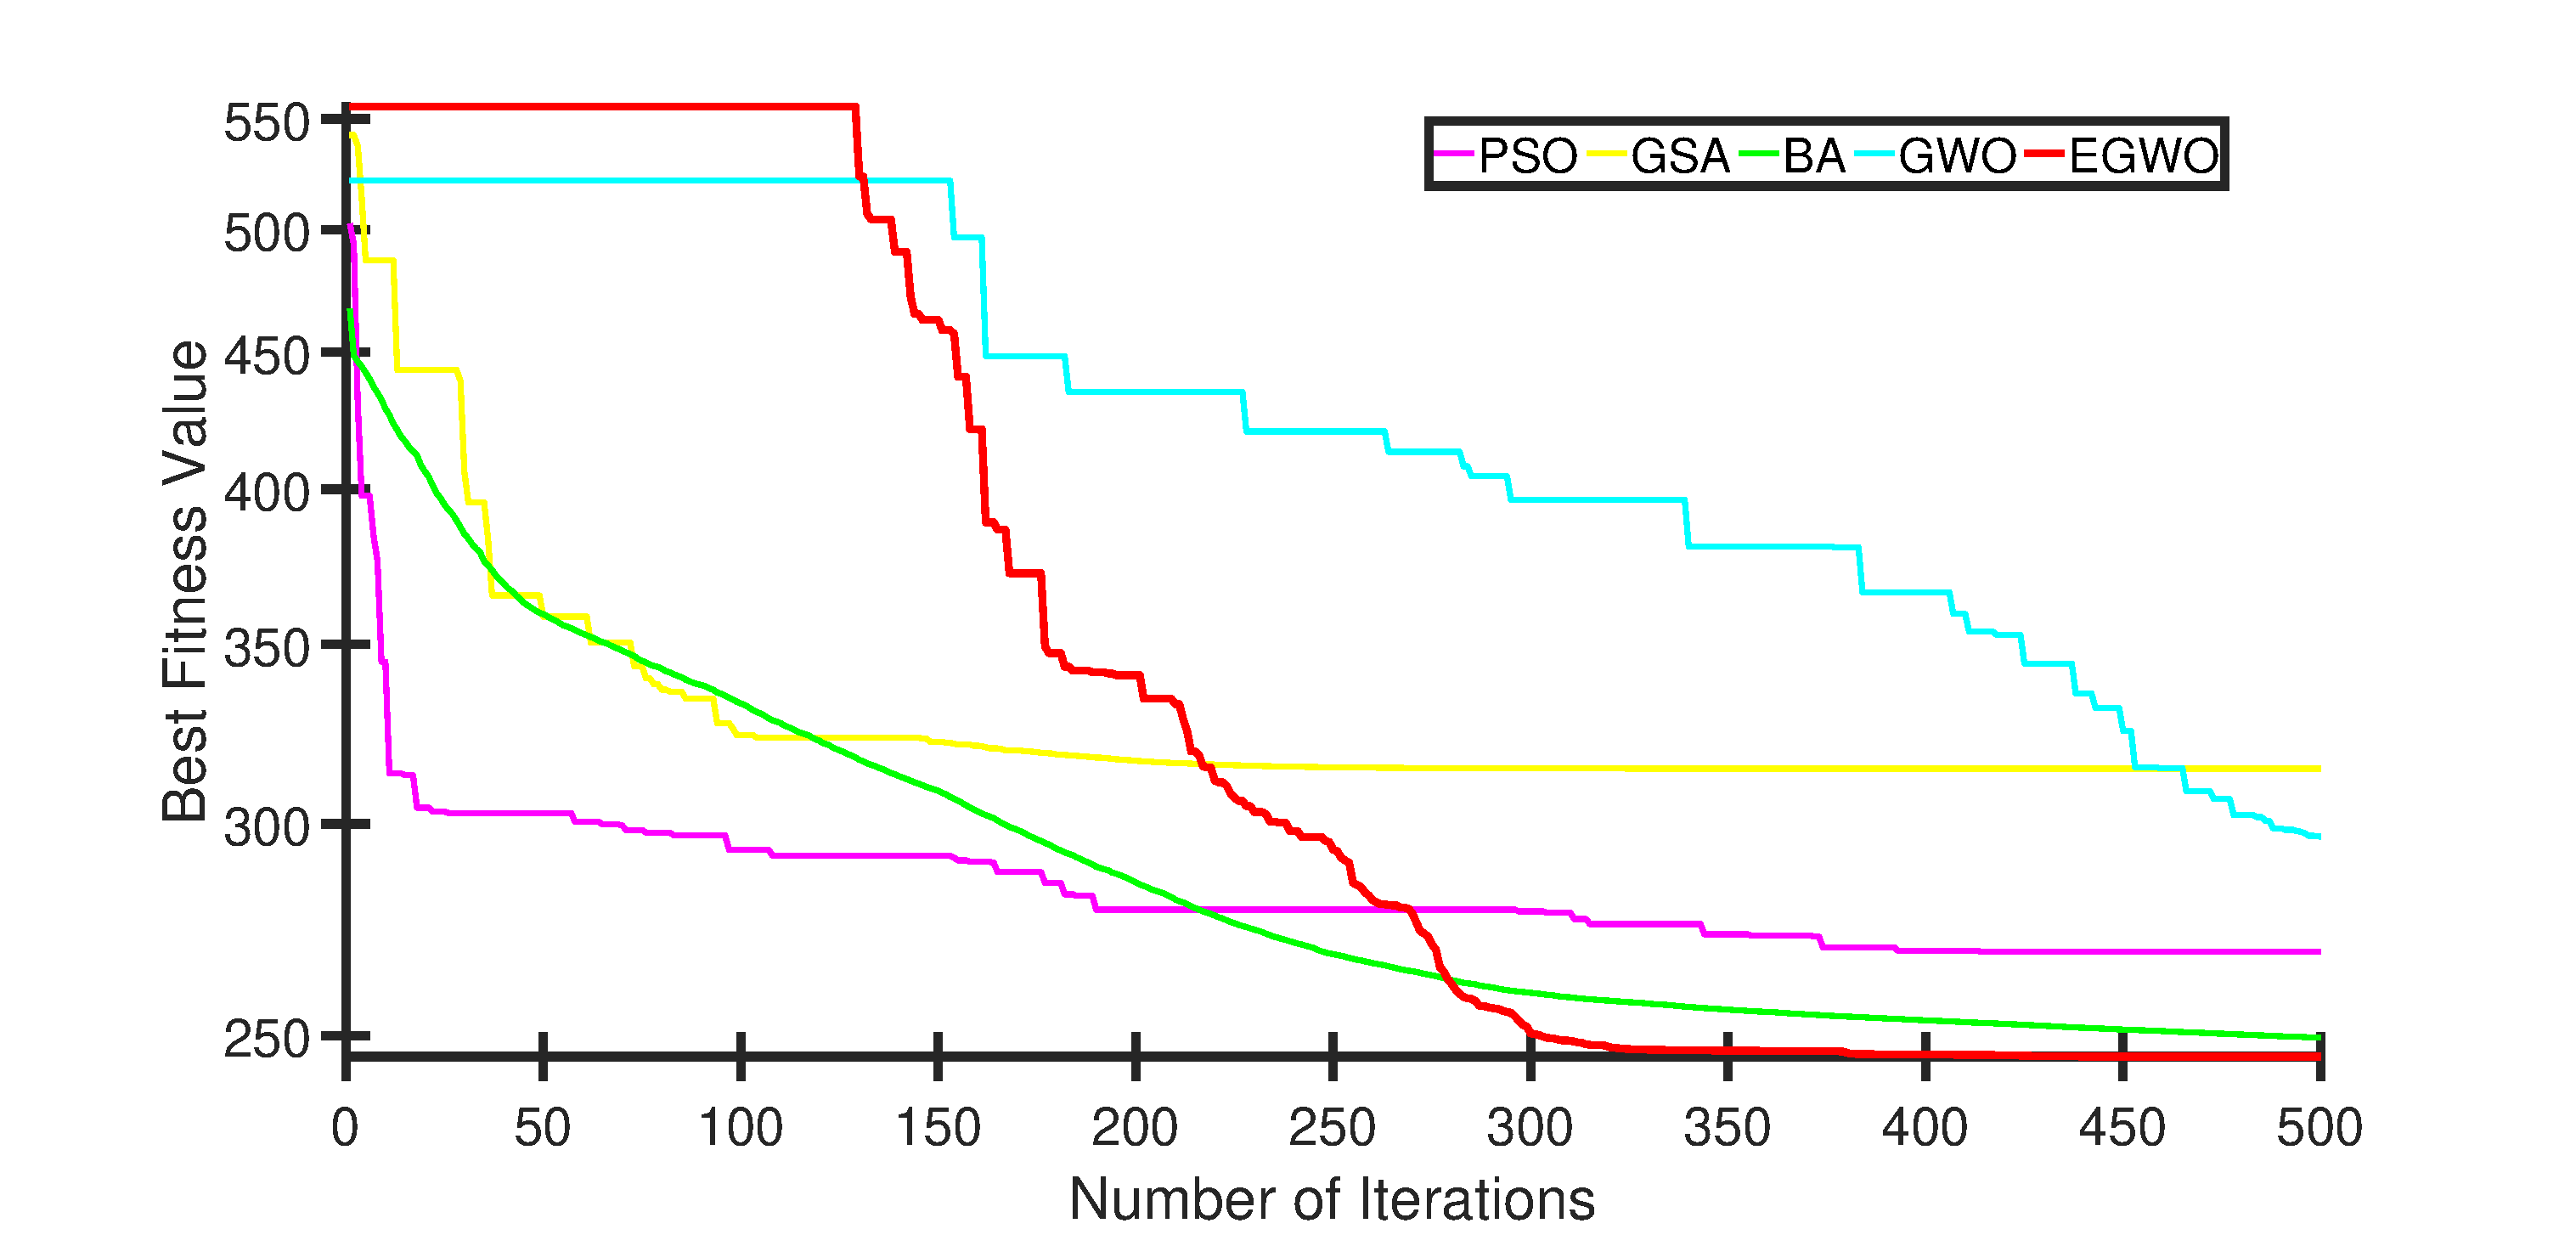
\includegraphics[width=2.8in,height=4.0cm]{CSheet4}}


     \caption{\small{The convergence graphs of (a) Wine and  (b) Glass }}
 \label{fig:ConvergenceGraph1}
\end{figure*}

\begin{figure*} 
   
    \subfigure[]{\includegraphics[width=2.8in,height=4.0cm]{Sheet2}}
     \subfigure[]{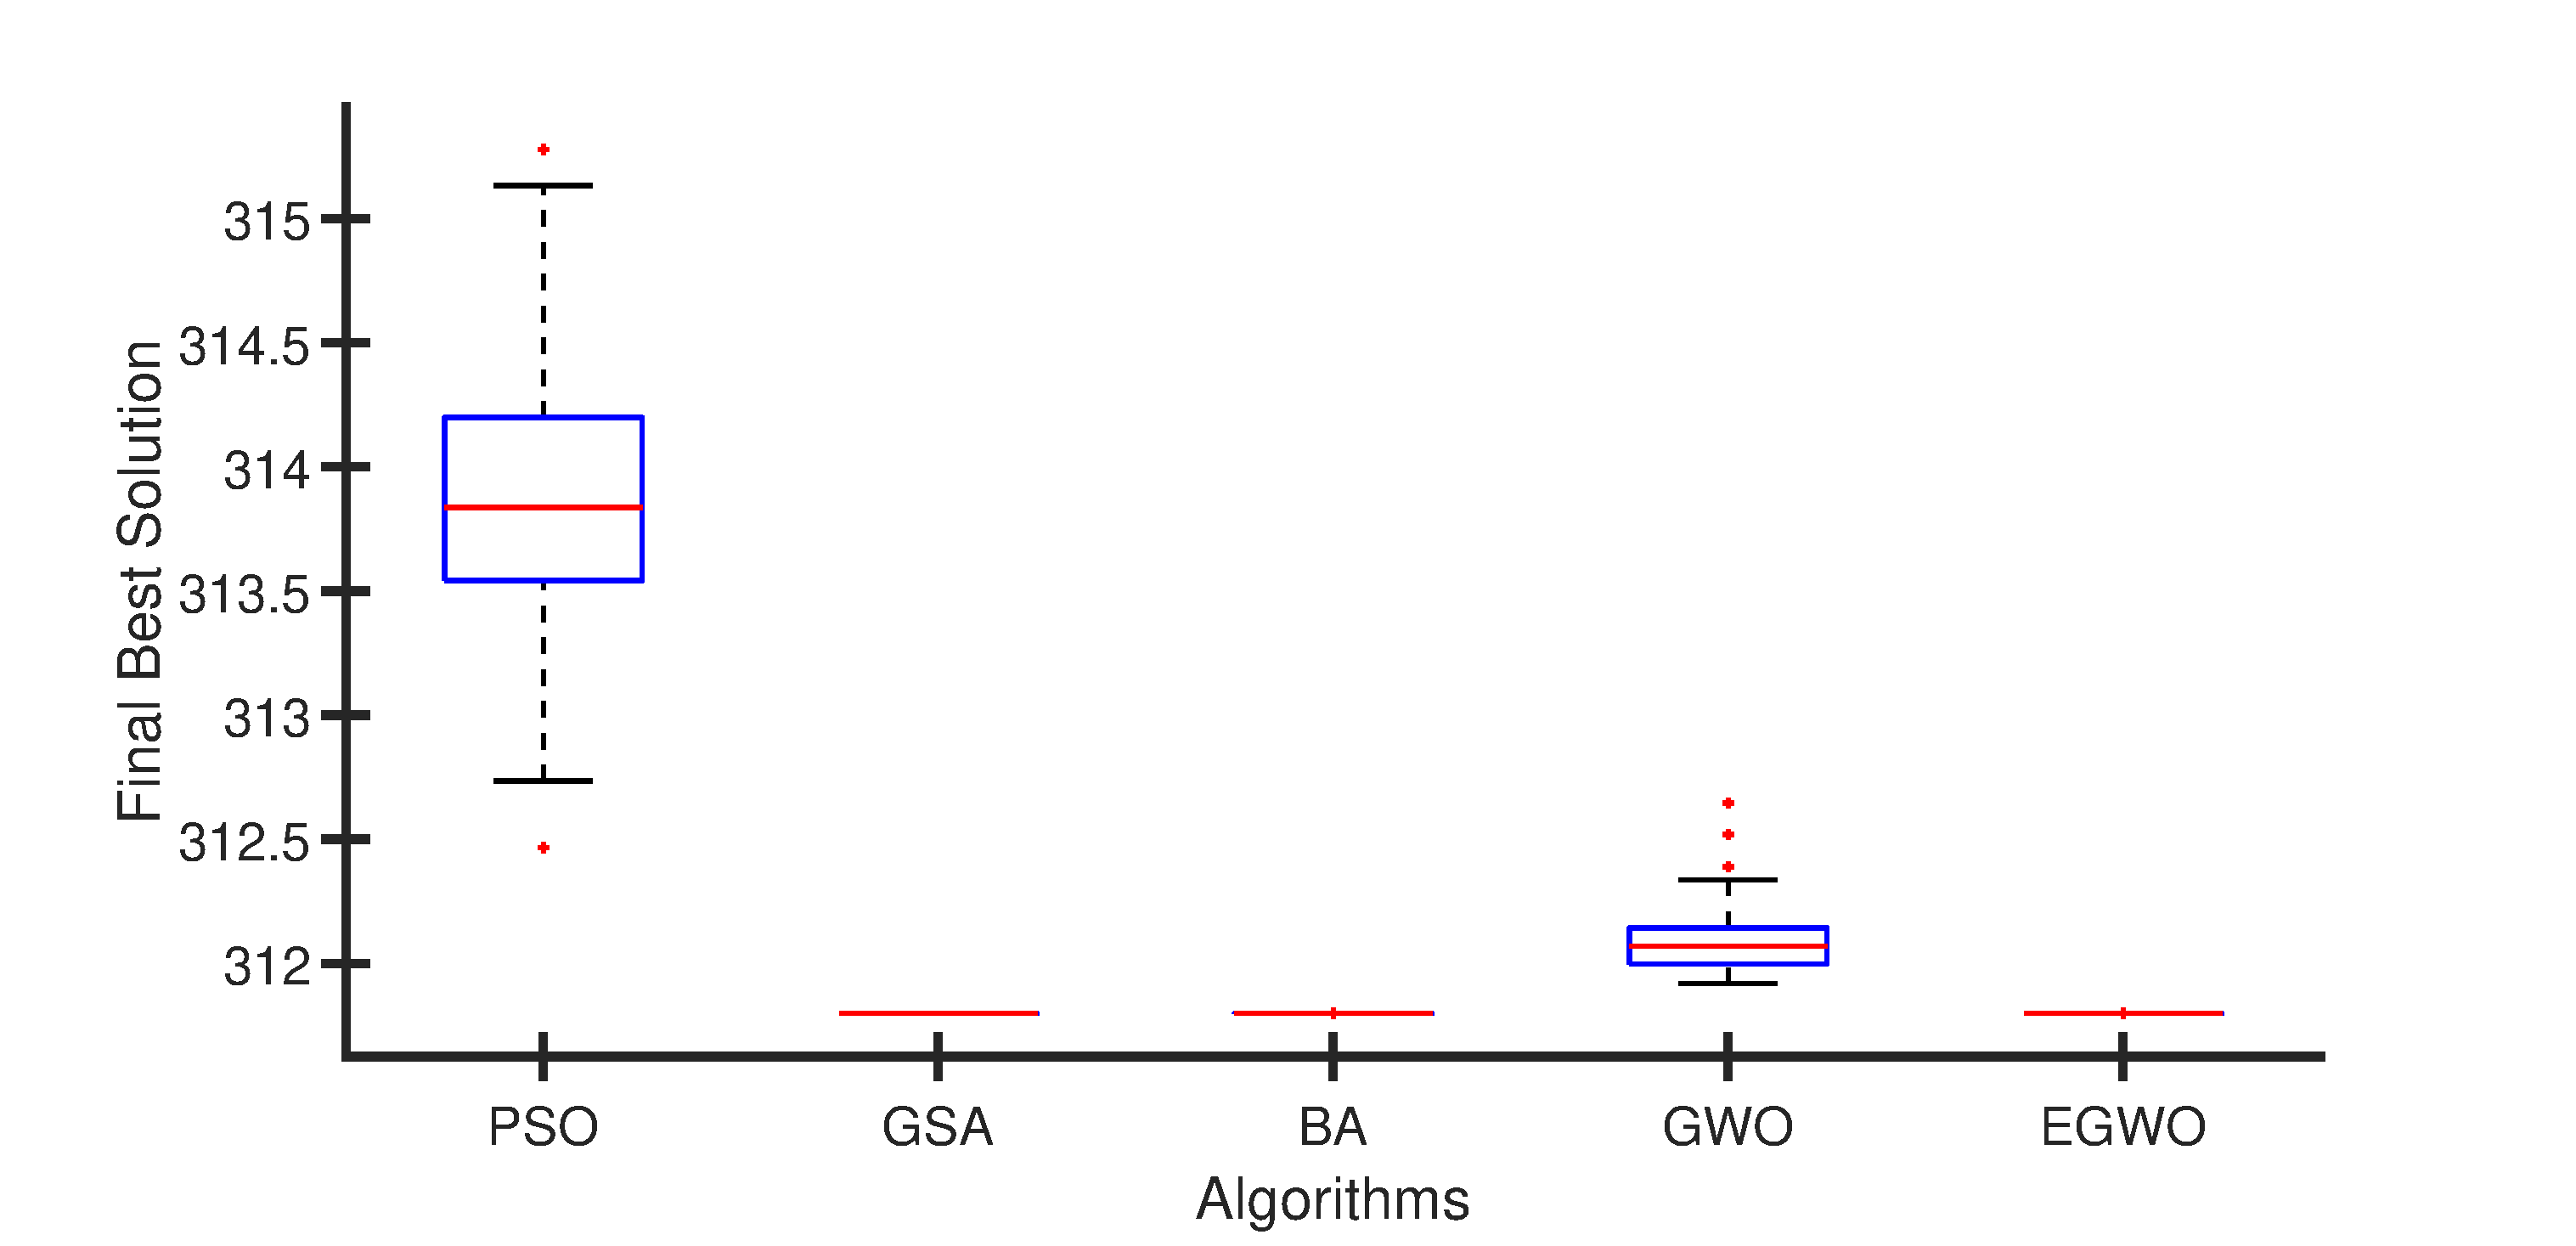
\includegraphics[width=2.8in,height=4.0cm]{Sheet3}}

    
      \caption{\small {The box-plot graphs for (a) Wine and  (b) Glass}}
\label{fig:Boxplot1}
\end{figure*}

\subsection{Performance analysis of MapReduce Based EGWO (MR-EGWO)}\label{sec:expr2}
In section \ref{sec:expr1}, EGWO has shown to be an efficient alternative for clustering task. Thus, the performance analysis of the parallelized EGWO, (MR-EGWO), is analyzed. Four large-scale synthetic datasets are used by duplicating each record of the original dataset $10^7$ times. Table \ref{tab:dataset} briefs these datasets in terms of three parameters, namely, number of actual clusters ($\#C$), number of dimensions ($\#D$) and number of data-points ($\#N$). The required parameter setting of all the method is same as given in Table \ref{tab:Param}.
For simulation, a Hadoop cluster of five nodes is designed where each node consists of an Intel Corei3-4570 processor with 3.20GHz, 4GB memory and 500 GB hard disk. Apache Hadoop version 2.6.2, java version 1.8.0 is used for the implementation of all methods and operating system is Ubuntu (operating system) version 14.04. 
Table \label{tab:FM} shows the values of F-measure obtained by each algorithm on four large scale synthetic datasets. The F-measure comparison of four MapRedcue based algorithms as given in Table \ref{tab:FM} confirms that the proposed MR-EGWO outperformed all the algorithms under comparison. Thus, it can be concluded that the proposed method can be used for efficient clustering of large datasets.

Furthermore, the speedup performance of the MR-EGWO is analyzed on iris and CMC datasets. The speedup measure of a method is determined by Eq. (\ref{eq:20}).
  \begin{equation}\label{eq:20}                                                            			
       S_p=T_{base}/T_N                                                     		
   \end{equation}
where, $T_{base}$ is the running time when $p$ method runs on one machine and $T_N$ is the running time of the same method on a cluster with $N$ machines. To measure the speedup performance of MR-EGWO, one machine is increased in the cluster on each run. The speedup performance of MR-EGWO is in illustrated in Fig. \ref{fig:Speedup}. It can be concluded from the Fig. \ref{fig:Speedup} that the running time of MR-EGWO decreases gradually with the increase of machines in the Hadoop cluster. Therefore, it is affirmed that the proposed MR-EGWO is advantageous for large-scale data.

\begin{table}
\caption{Large Datasets}
\scriptsize
\begin{center}
\renewcommand{\arraystretch}{0.7}
  \begin{tabular}{l l l l }

    \hline
\textbf{Dataset} & \textbf{\#C} & \textbf{\#D} 		&		\textbf{\#N}    \\
\hline
 Replicated Iris	&	3	&	7	&	10,000,050	\\
Replicated CMC	&	3	&	9	&	10,000,197	\\
Replicated Wine	&	2	&	18	&	5000000	\\
Replicated Vovel &	10	& 10	&	1025010	\\

    \hline
  \end{tabular}
\end{center}
\label{tab:large dataset}
\end{table}


\begin{table}
\caption{F-Measure results obtained by the MapReduce based algorithms}
\scriptsize
\begin{center}
\renewcommand{\arraystretch}{0.7}
  \begin{tabular}{l l l l l l l}
    \hline
    \hline
\textbf{Data set} & \textbf{PK-Means} &\textbf{parallel KPSO} &\textbf{MR-ABC} &\textbf{DFBPKBA} &\textbf{MR-EGWO}\\
\hline

1	&	0.667	&	0.785	&	0.842	&	0.790  &  0.846	\\
2	&	0.298	&	0.324	&	0.387	&	0.378  &  0.391	\\
3	&	0.482	&	0.517	&	0.718	&	0.719  &  0.733	\\
4	&	0.586	&	0.627	&	0.634	&	0.622  &  0.635	\\

    \hline
  \end{tabular}
\end{center}
\label{tab:FM}
\end{table}



\begin{figure}
    \centering

     \subfigure[]{\includegraphics[width=2.0in,height=3.5cm]{iris}}
     \subfigure[]{\includegraphics[width=2.0in,height=3.5cm]{cmc}}
    
     \caption{\small{The speedup graph of  (a) Iris (b) CMC}}
 \label{fig:Speedup}
\end{figure}
 

\section{Conclusion}\label{sec:con}

In this paper, a novel MapReduce based clustering method is presented. The proposed method has three folds, (i) An efficient variant of grey-wolf optimizer called enhanced grey-wolf optimizer (EGWO) has been introduced for improving the quality of clustering (ii) The performance of the proposed variant (EGWO) is validated on seven benchmark datasets for clustering problem. The proposed method has outperformed five clustering methods namely: K-means, PSO, GSA, BA and GWO in terms of mean and best fitness values. The exploration and exploitation capabilities of the proposed variant are also analyzed using convergence graph. Boxplots are drawn to study the consistency of the results over the 30 runs. Third, a novel method named, MR-EGWO is proposed by parallelizing the EGWO using MapReduce for clustering large scale data sets. The proposed method, MR-EGWO, takes the advantage of EGWO to alleviate the clustering quality and MapReduce architecture to cope with large scale datasets. Furthermore, to ascertain the efficiency of the MR-EGWO in the parallel environment, the proposed method is run on the Hadoop cluster of five nodes for four large scale synthetic datasets namely, iris, CMC, wine, and vovel. The simulation results outperformed four state-of-the-art MapReduce based clustering methods in terms of F-measure. Moreover, the speedup efficiency of the MR-EGWO is studied on two synthetic datasets (iris and CMC) by varying the number of nodes of the Hadoop cluster. The speedup results show that MR-EGWO is well suited for analyzing large datasets with significant speedup performance and better clustering quality. Thus, it is concluded that MR-EGWO is a competitive method for large scale clustering problems. In future, the work may be extended to test on real world clustering applications with large datasets.\\
\textbf{References}



\bibliographystyle{elsarticle-num}
\begin{thebibliography}{10}
\expandafter\ifx\csname url\endcsname\relax
  \def\url#1{\texttt{#1}}\fi
\expandafter\ifx\csname urlprefix\endcsname\relax\def\urlprefix{URL }\fi
\expandafter\ifx\csname href\endcsname\relax
  \def\href#1#2{#2} \def\path#1{#1}\fi

\bibitem{fayyad2002information}
U.~M. Fayyad, A.~Wierse, G.~G. Grinstein, Information visualization in data
  mining and knowledge discovery, Morgan Kaufmann, 2002.

\bibitem{friedman2007anomaly}
M.~Friedman, M.~Last, Y.~Makover, A.~Kandel, Anomaly detection in web documents
  using crisp and fuzzy-based cosine clustering methodology, Information
  sciences 177 (2007) 467--475.

\bibitem{liao2008mri}
L.~Liao, T.~Lin, B.~Li, Mri brain image segmentation and bias field correction
  based on fast spatially constrained kernel clustering approach, Pattern
  Recognition Letters 29 (2008) 1580--1588.

\bibitem{forgy1965cluster}
E.~W. Forgy, Cluster analysis of multivariate data: efficiency versus
  interpretability of classifications, Biometrics 21 (1965) 768--769.

\bibitem{xu2005}
R.~Xu, D.~Wunsch, Survey of clustering algorithms, IEEE Transactions on neural
  networks 16 (2005) 645--678.

\bibitem{kaufman2009finding}
L.~Kaufman, P.~J. Rousseeuw, Finding groups in data: an introduction to cluster
  analysis, Vol. 344, John Wiley \& Sons, 2009.

\bibitem{kao2008hybridized}
Y.-T. Kao, E.~Zahara, I.-W. Kao, A hybridized approach to data clustering,
  Expert Systems with Applications 34~(3) (2008) 1754--1762.

\bibitem{maulik2000genetic}
U.~Maulik, S.~Bandyopadhyay, Genetic algorithm-based clustering technique,
  Pattern recognition 33~(9) (2000) 1455--1465.

\bibitem{karaboga2011novel}
D.~Karaboga, C.~Ozturk, A novel clustering approach: Artificial bee colony
  (abc) algorithm, Applied soft computing 11~(1) (2011) 652--657.

\bibitem{alam2008particle}
S.~Alam, G.~Dobbie, P.~Riddle, Particle swarm optimization based clustering of
  web usage data, in: Proceedings of the 2008 IEEE/WIC/ACM International
  Conference on Web Intelligence and Intelligent Agent Technology-Volume 03,
  IEEE Computer Society, 2008, pp. 451--454.
\bibitem{ashish2018parallel}
T.~Ashish, S.~Kapil, B.~Manju, Parallel bat algorithm-based clustering using
  mapreduce, in: Networking Communication and Data Knowledge Engineering,
  Springer, 2018, pp. 73--82.

\bibitem{kumar2017grey}
V.~Kumar, J.~K. Chhabra, D.~Kumar, Grey wolf algorithm-based clustering
  technique, Journal of Intelligent Systems 26~(1) (2017) 153--168.
\bibitem{hatamlou2012combined}
A.~Hatamlou, S.~Abdullah, H.~Nezamabadi-Pour, A combined approach for
  clustering based on k-means and gravitational search algorithms, Swarm and
  Evolutionary Computation 6 (2012) 47--52.

\bibitem{shvachko2010hadoop}
K.~Shvachko, H.~Kuang, S.~Radia, R.~Chansler, The hadoop distributed file
  system, in: 2010 IEEE 26th symposium on mass storage systems and technologies
  (MSST), IEEE, 2010, pp. 1--10.

\bibitem{FrontPag86:online}
Frontpage - hadoop wiki, \url{http://wiki.apache.org/hadoop/}, (Accessed on
  09/17/2016).

\bibitem{dean2008mapreduce}
J.~Dean, S.~Ghemawat, Mapreduce: simplified data processing on large clusters,
  Communications of the ACM 51~(1) (2008) 107--113.

\bibitem{khezr2015mapreduce}
S.~N. Khezr, N.~J. Navimipour, Mapreduce and its application in optimization
  algorithms: A comprehensive study, Majlesi Journal of Multimedia Processing
  4~(3).
\bibitem{wolpert1997no}
D.~H. Wolpert, W.~G. Macready, No free lunch theorems for optimization, IEEE
  transactions on evolutionary computation 1~(1) (1997) 67--82.

\bibitem{wang2012parallel}
J.~Wang, D.~Yuan, M.~Jiang, Parallel k-pso based on mapreduce, in:
  Communication Technology (ICCT), 2012 IEEE 14th International Conference on,
  IEEE, 2012, pp. 1203--1208.

\bibitem{lin2013parallelizing}
C.-Y. Lin, Y.-M. Pai, K.-H. Tsai, C.~H.-P. Wen, L.-C. Wang, Parallelizing
  modified cuckoo search on mapreduce architecture, Journal of Electronic
  Science and Technology 11~(2) (2013) 115--123.

\bibitem{gong2015distributed}
Y.-J. Gong, W.-N. Chen, Z.-H. Zhan, J.~Zhang, Y.~Li, Q.~Zhang, J.-J. Li,
  Distributed evolutionary algorithms and their models: A survey of the
  state-of-the-art, Applied Soft Computing 34 (2015) 286--300.

\bibitem{meena2012enhanced}
M.~J. Meena, K.~Chandran, A.~Karthik, A.~V. Samuel, An enhanced aco algorithm
  to select features for text categorization and its parallelization, Expert
  Systems with Applications 39~(5) (2012) 5861--5871.

\bibitem{aljarah2013towards}
I.~Aljarah, S.~A. Ludwig, Towards a scalable intrusion detection system based
  on parallel pso clustering using mapreduce, in: Proceedings of the 15th
  annual conference companion on Genetic and evolutionary computation, ACM,
  2013, pp. 169--170.

\bibitem{wu2012mapreduce}
B.~Wu, G.~Wu, M.~Yang, A mapreduce based ant colony optimization approach to
  combinatorial optimization problems, in: Natural Computation (ICNC), 2012
  Eighth International Conference on, IEEE, 2012, pp. 728--732.

\bibitem{xu2014novel}
X.~Xu, Z.~Ji, F.~Yuan, X.~Liu, A novel parallel approach of cuckoo search using
  mapreduce, in: 2014 International Conference on Computer, Communications and
  Information Technology (CCIT 2014), Atlantis Press, 2014.

\bibitem{moertini2016enhancing}
V.~S. Moertini, L.~Venica, Enhancing parallel k-means using map reduce for
  discovering knowledge from big data, in: 2016 IEEE International Conference
  on Cloud Computing and Big Data Analysis (ICCCBDA), IEEE, 2016, pp. 81--87.
\bibitem{banharnsakun2016mapreduce}
A.~Banharnsakun, A mapreduce-based artificial bee colony for large-scale data
  clustering, Pattern Recognition Letters.

\bibitem{feoktistov2007differential}
V.~Feoktistov, Differential evolution: in search of solutions, Vol.~5, Springer
  Science \& Business Media, 2007.

\bibitem{tripathidynamic}
A.~K. Tripathi, K.~Sharma, M.~Bala, Dynamic frequency based parallel k-bat
  algorithm for massive data clustering (dfbpkba), International Journal of
  System Assurance Engineering and Management  1--9.

\bibitem{zhao2009parallel}
W.~Zhao, H.~Ma, Q.~He, Parallel k-means clustering based on mapreduce, in: IEEE
  International Conference on Cloud Computing, Springer, 2009, pp. 674--679.





\bibitem{brown2007levy}
C.~T. Brown, L.~S. Liebovitch, R.~Glendon, L{\'e}vy flights in dobe ju/’hoansi
  foraging patterns, Human Ecology 35~(1) (2007) 129--138.

\bibitem{reynolds2007free}
A.~M. Reynolds, M.~A. Frye, Free-flight odor tracking in drosophila is
  consistent with an optimal intermittent scale-free search, PloS one 2~(4)
  (2007) e354.

\bibitem{pavlyukevich2007levy}
I.~Pavlyukevich, L{\'e}vy flights, non-local search and simulated annealing,
  Journal of Computational Physics 226~(2) (2007) 1830--1844.

\bibitem{yang2010evolutionary}
S.~Yang, R.~Wu, M.~Wang, L.~Jiao, Evolutionary clustering based vector
  quantization and spiht coding for image compression, Pattern Recognition
  Letters 31~(13) (2010) 1773--1780.

\bibitem{shlesinger1995levy}
M.~F. Shlesinger, G.~M. Zaslavsky, U.~Frisch, L{\'e}vy flights and related
  topics in physics, Lecture notes in physics 450 (1995) 52.

\bibitem{mirjalili2014grey}
S.~Mirjalili, S.~M. Mirjalili, A.~Lewis, Grey wolf optimizer, Advances in
  Engineering Software 69 (2014) 46--61.


\bibitem{zhang2015grey}
S.~Zhang, Y.~Zhou, Grey wolf optimizer based on powell local optimization
  method for clustering analysis, Discrete Dynamics in Nature and Society 2015.

\bibitem{yang2010eagle}
X.-S. Yang, S.~Deb, Eagle strategy using l{\'e}vy walk and firefly algorithms
  for stochastic optimization, Nature Inspired Cooperative Strategies for
  Optimization (NICSO 2010) (2010) 101--111.

\bibitem{blake1998uci}
C.~Blake, C.~J. Merz, $\{$UCI$\}$ repository of machine learning databases.

\bibitem{heidari2017efficient}
A.~A. Heidari, P.~Pahlavani, An efficient modified grey wolf optimizer with
  l{\'e}vy flight for optimization tasks, Applied Soft Computing 60 (2017)
  115--134.





\bibitem{emary2016binary}
E.~Emary, H.~M. Zawbaa, A.~E. Hassanien, Binary grey wolf optimization
  approaches for feature selection, Neurocomputing 172 (2016) 371--381.

\bibitem{jayabarathi2016economic}
T.~Jayabarathi, T.~Raghunathan, B.~Adarsh, P.~N. Suganthan, Economic dispatch
  using hybrid grey wolf optimizer, Energy 111 (2016) 630--641.

\bibitem{medjahed2016gray}
S.~A. Medjahed, T.~A. Saadi, A.~Benyettou, M.~Ouali, Gray wolf optimizer for
  hyperspectral band selection, Applied Soft Computing 40 (2016) 178--186.

\bibitem{jayakumar2016grey}
N.~Jayakumar, S.~Subramanian, S.~Ganesan, E.~Elanchezhian, Grey wolf
  optimization for combined heat and power dispatch with cogeneration systems,
  International Journal of Electrical Power \& Energy Systems 74 (2016)
  252--264.

\bibitem{komaki2015grey}
G.~Komaki, V.~Kayvanfar, Grey wolf optimizer algorithm for the two-stage
  assembly flow shop scheduling problem with release time, Journal of
  Computational Science 8 (2015) 109--120.

\bibitem{guha2016load}
D.~Guha, P.~K. Roy, S.~Banerjee, Load frequency control of interconnected power
  system using grey wolf optimization, Swarm and Evolutionary Computation 27
  (2016) 97--115.

\bibitem{ho2002simple}
Y.-C. Ho, D.~L. Pepyne, Simple explanation of the no-free-lunch theorem and its
  implications, Journal of optimization theory and applications 115~(3) (2002)
  549--570.

\bibitem{el2015single}
A.~A. El-Fergany, H.~M. Hasanien, Single and multi-objective optimal power flow
  using grey wolf optimizer and differential evolution algorithms, Electric
  Power Components and Systems 43~(13) (2015) 1548--1559.

\bibitem{shakarami2016wide}
M.~Shakarami, I.~F. Davoudkhani, Wide-area power system stabilizer design based
  on grey wolf optimization algorithm considering the time delay, Electric
  Power Systems Research 133 (2016) 149--159.




\end{thebibliography}



\end{document}











